\section{Results}

\subsection{Average Time Between Samples}
I did this for all benchmarks, but didn't parse and calculate individual averages per benchmarks. Just did average across benchmark, grouped by monitor type.
    \begin{figure}[H]
    	\centering
    	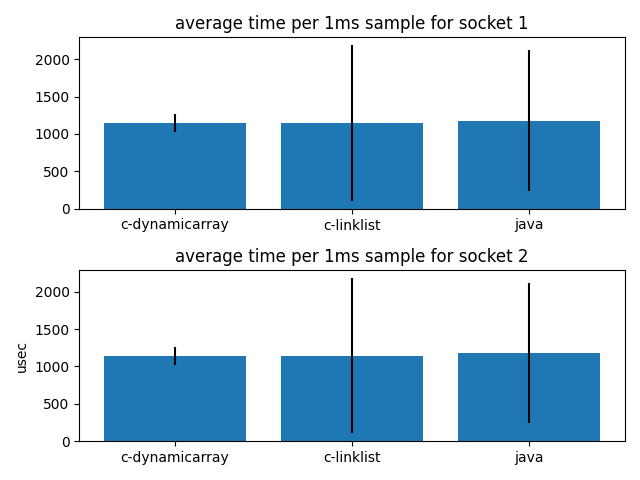
\includegraphics[width=17cm,height=17cm,keepaspectratio]{AsyncMonitorCompares/time-energy-persample/timestamp_average_usec_per-sample.png}
    	\caption{average reported usecs between 1 msec sample}
   	\label{fig:xalan-PKG-Time-scatter}
    \end{figure}

\subsection{Average Sample Energy}
I did this for all benchmarks, but didn't parse and calculate individual averages per benchmarks. Just did average across benchmark, grouped by monitor type.
    \begin{figure}[H]
    	\centering
    	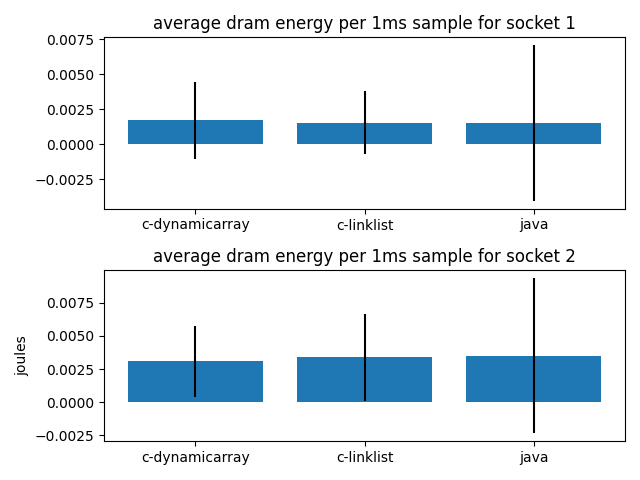
\includegraphics[width=17cm,height=17cm,keepaspectratio]{AsyncMonitorCompares/time-energy-persample/dram_average_joules_per-sample.png}
    	\caption{average energy per sample for dram}
   	\label{fig:xalan-PKG-Time-scatter}
    \end{figure}
    \begin{figure}[H]
    	\centering
    	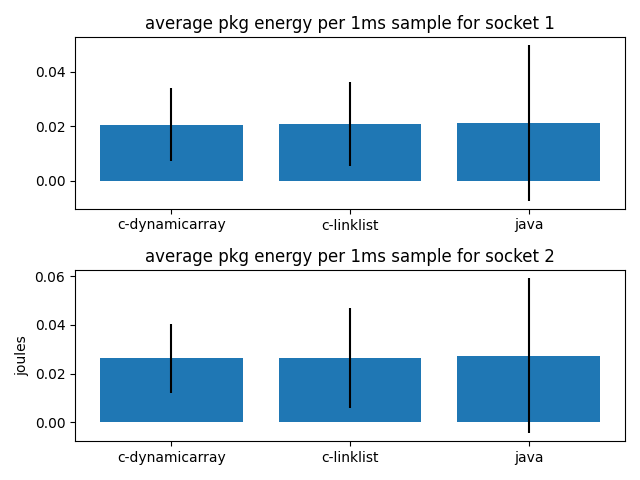
\includegraphics[width=17cm,height=17cm,keepaspectratio]{AsyncMonitorCompares/time-energy-persample/pkg_average_joules_per-sample.png}
    	\caption{average energy per sample for pkg}
   	\label{fig:xalan-PKG-Time-scatter}
    \end{figure}
    
\subsection{JNI Runtime Overhead}
    The graphs below are histograms. X axis is the microsecond runtimes, Y axis is how many readings we got
    for that runtime. Crazy high values (more than 3 standard deviations from the mean) are removed because they are relatively few and that stretch the graph and make it illegible. But we still captured
    them in the Python script, because they're probably important information and intend to render them somehow.

    It appears that creating a \texttt{jstring} and rendering it in Java as a \texttt{String} is has notable time overhead and variance as well.
    
    It seems that while a JNI call itself does not incur overhead, as demonstrated with similar runtimes for our void-returning native methods, our method that returns a string of energy data has a considerable runtime increase from simply calling the C side function. So creation of a Java string in C, and then passing it to Java, provides a notable cost, both in time of execution and in variance of the time. \todo{finalize the results from that recent test you did, see how it goes in terms of substantiating this}
    
    \anote{Should I also note that on my 1-socket computer the JNI overhead is a lot lower? It's probably because I'm returning less data, so the object I build is smaller.}
    
    \begin{figure}[H]
	    \centering
	    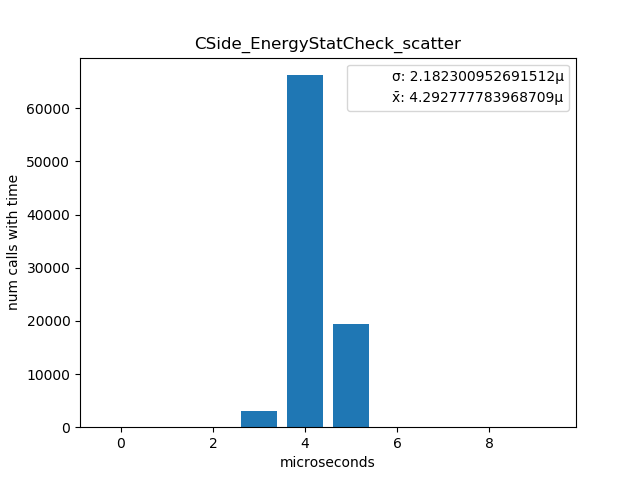
\includegraphics[width=10cm,height=10cm,keepaspectratio]{jmh/jni-overhead/CSide_EnergyStatCheck_scatter.png}
	    \caption{Runtime for EnergyStatCheck on CSide}
	    \label{fig:jolteon-jmh-runtime-energystatcheck-c}
    \end{figure}
    \begin{figure}[H]
	    \centering
	    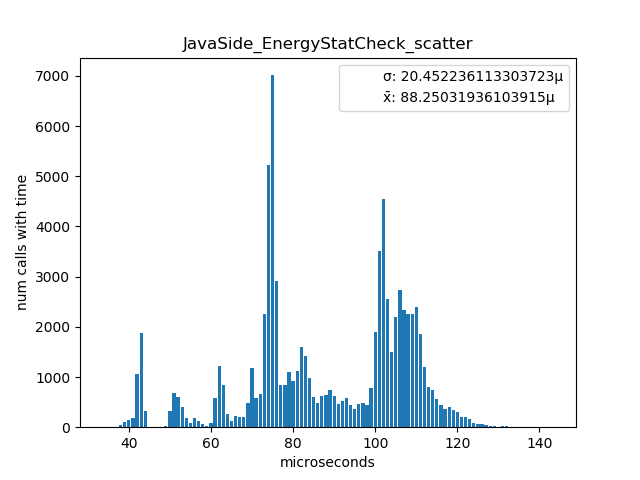
\includegraphics[width=10cm,height=10cm,keepaspectratio]{jmh/jni-overhead/JavaSide_EnergyStatCheck_scatter.png}
	    \caption{Runtime for EnergyStatCheck on JavaSide}
	    \label{fig:jolteon-jmh-runtime-energystatcheck-java}
    \end{figure}
    
    \begin{figure}[H]
	    \centering
	    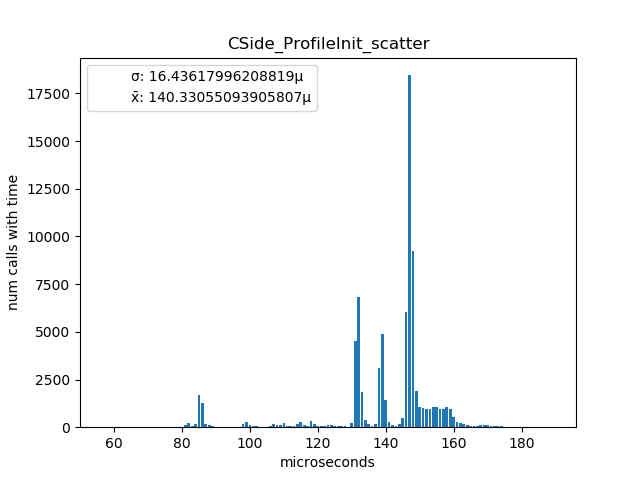
\includegraphics[width=10cm,height=10cm,keepaspectratio]{jmh/jni-overhead/CSide_ProfileInit_scatter.png}
	    \caption{Runtime for ProfileInit on CSide}
	    \label{fig:jolteon-jmh-runtime-profileinit-c}
    \end{figure}
    \begin{figure}[H]
	    \centering
	    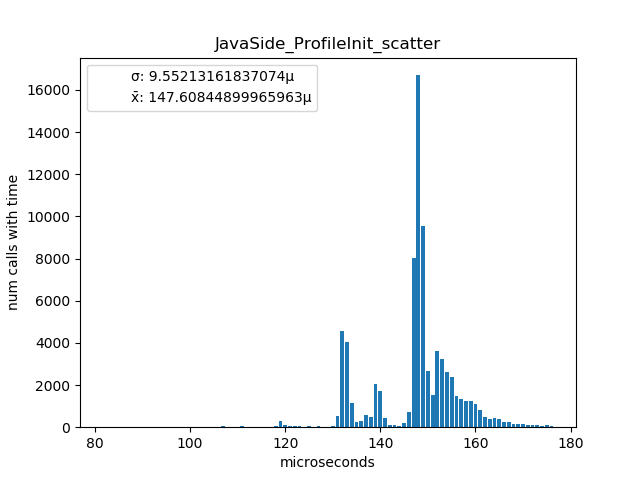
\includegraphics[width=10cm,height=10cm,keepaspectratio]{jmh/jni-overhead/JavaSide_ProfileInit_scatter.png}
	    \caption{Runtime for ProfileInit on JavaSide}
	    \label{fig:jolteon-jmh-runtime-profileinit-java}
    \end{figure}

    \begin{figure}[H]
	    \centering
	    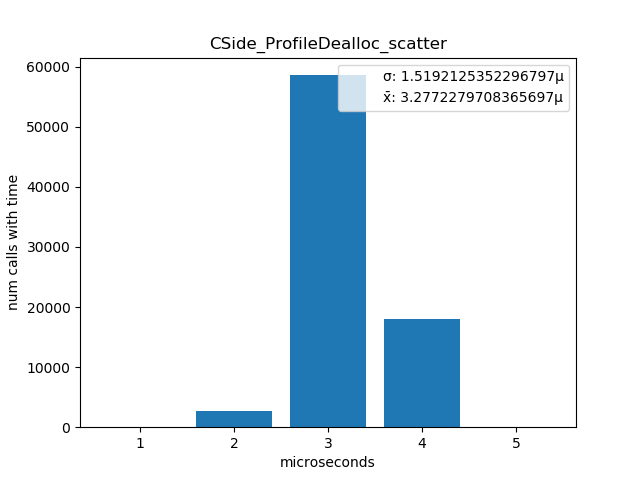
\includegraphics[width=10cm,height=10cm,keepaspectratio]{jmh/jni-overhead/CSide_ProfileDealloc_scatter.png}
	    \caption{Runtime for ProfileDealloc on CSide}
	    \label{fig:jolteon-jmh-runtime-profileDealloc-c}
    \end{figure}
    \begin{figure}[H]
	    \centering
	    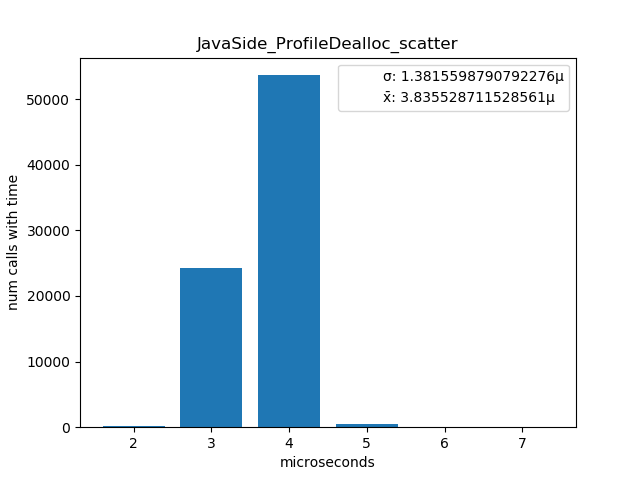
\includegraphics[width=10cm,height=10cm,keepaspectratio]{jmh/jni-overhead/JavaSide_ProfileDealloc_scatter.png}
	    \caption{Runtime for ProfileDealloc on JavaSide}
	    \label{fig:jolteon-jmh-runtime-profileDealloc-java}
    \end{figure}

\subsection{Time to Read One Energy Value from MSR}
    It's all hovering around one microsecond, with occasional relatively-high values. Values greater than 3 standard deviations weren't plotted because it makes the graph illegible, but we still captured them
    in the Python script and intend to represent them somehow, because it's still probably good to know
    that we'll very occasionally get super high runtimes.
    
    Graphs below are histograms. X axis is the runtime, Y axis is how many readings we found at that runtime.
    
    \begin{figure}[H]
	    \centering
	    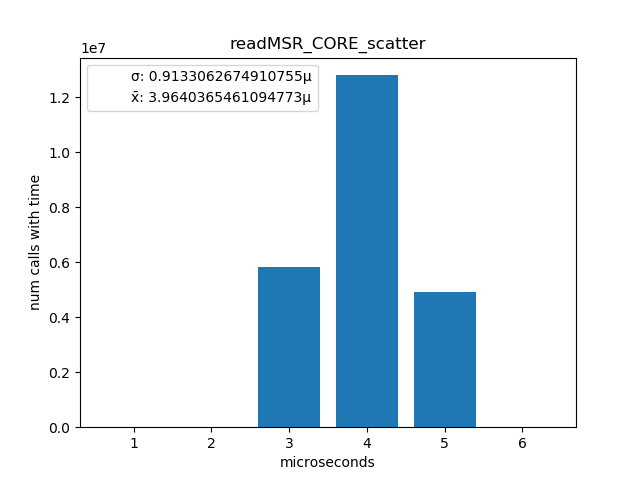
\includegraphics[width=10cm,height=10cm,keepaspectratio]{jmh/readmsr-runtime/readMSR_CORE_scatter.png}
	    \caption{Runtime to read MSR for CORE RAPL counter}
	    \label{fig:CORE-rapl-counter}
    \end{figure}
    
    \begin{figure}[H]
	    \centering
	    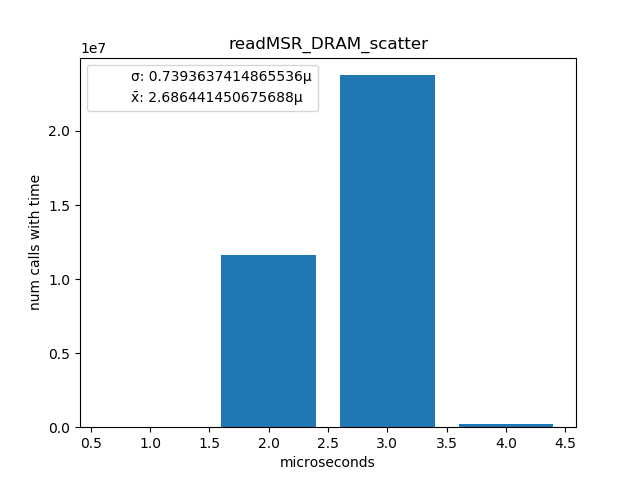
\includegraphics[width=10cm,height=10cm,keepaspectratio]{jmh/readmsr-runtime/readMSR_DRAM_scatter.png}
	    \caption{Runtime to read MSR for DRAM RAPL counter}
	    \label{fig:DRAM-rapl-counter}
    \end{figure}
    
    \begin{figure}[H]
	    \centering
	    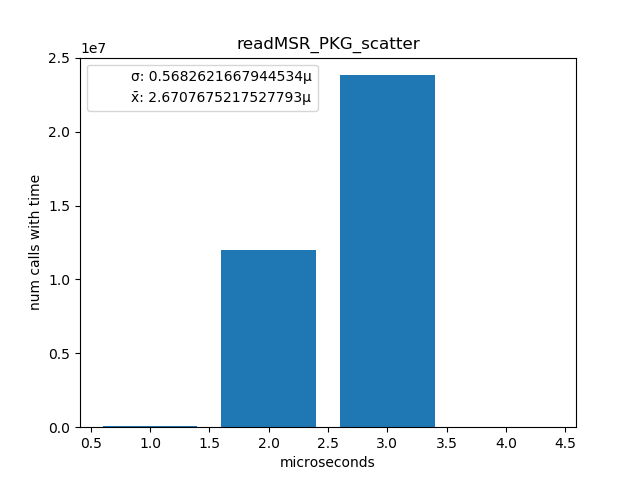
\includegraphics[width=10cm,height=10cm,keepaspectratio]{jmh/readmsr-runtime/readMSR_PKG_scatter.png}
	    \caption{Runtime to read MSR for PKG RAPL counter}
	    \label{fig:PKG-rapl-counter}
    \end{figure}
    
    %\begin{figure}[H]
	%    \centering
	%    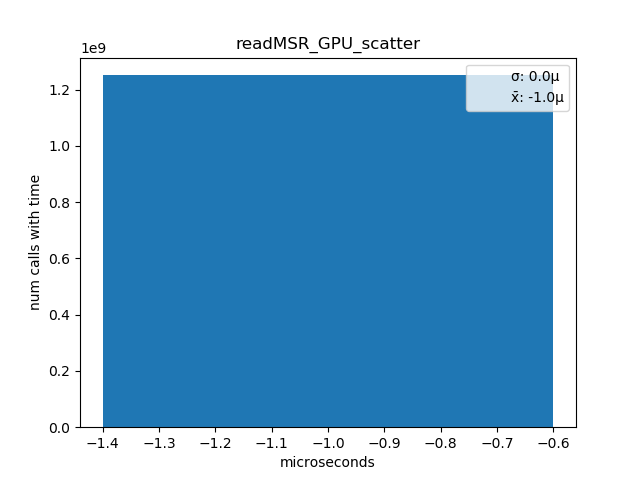
\includegraphics[width=10cm,height=10cm,keepaspectratio]{jmh/readmsr-runtime/readMSR_GPU_scatter.png}
	%    \caption{Runtime to read MSR for GPU RAPL counter}
	%    \label{fig:GPU-rapl-counter}
    %\end{figure}
    

\subsection{Java SyncEnergyMonitor Sampling Runtime}
This part is to show the runtime of taking a whole sample. This can serve to show the time overhead of simply taking a sample, the whole difference between Java and C for sampling (other experiments just isolate the JNI portion of the overhead), and the runtime of the three different types of samples that are taken: raw string sample, primitive array sample, and object sample.

Object sample vs primitive sample runtime is useful for people to know if they're thinking about the tradeoff. There's pretty clearly going to be a memory difference (obviously), but also runtime could be useful. (Make sure you confirm the difference in runtime that you just observed).

String sample is (maybe) relevant because Java Side Async Monitor directly stores the string samples, so we can compare this sampling runtime with the C side runtime. Can make for explanations about performance difference between C and Java side Async Monitors. However, this method is package private and we covered a close-enough situation in the JNI runtime overhead, so it might be better to just look at that.

JMH experiment: 7 warmups, 30 iterations, 10 second period for warmup and iteration. As many shots as possible per iteration (with 100-count busywait, so MSRs dont shut down), takes the average of the runtime in microseonds.

    \begin{figure}[H]
	    \centering
	    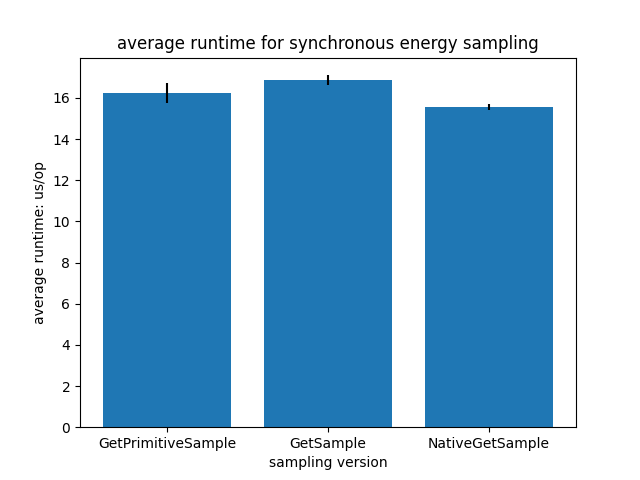
\includegraphics[width=10cm,height=10cm,keepaspectratio]{jmh/syncmonitor/sync-samples-runtime.png}
	    \caption{Runtimes per sampling function}
	    \label{fig:PKG-rapl-counter}
    \end{figure}

While there is a predictable difference in overhead run time, it is all within the range of a single microsecond. Memory could be a consideration for whether or not a primitive array or object wrapper should be used to represent an energy sample, but in most cases, runtime should not.

\subsection{AsyncEnergyMonitor Comparison}
\subsubsection{Sampling Efficiency}
Comparing how efficient the sampling is for each monitor. Divide number of samples collected
by msec lifetime of monitor. The first graph is average for the 20 benchmark iterations and
the second is average per monitor across all iterations.

    \begin{figure}[H]
    	\centering
    	\includegraphics[width=17cm,height=17cm,keepaspectratio]{AsyncMonitorCompares/sampling-efficiency_perbench.png}
    	\caption{Average sampling efficiency per benchmark}
    	\label{fig:samplingefficiency_perbench}
    \end{figure}
    \begin{figure}[H]
    	\centering
    	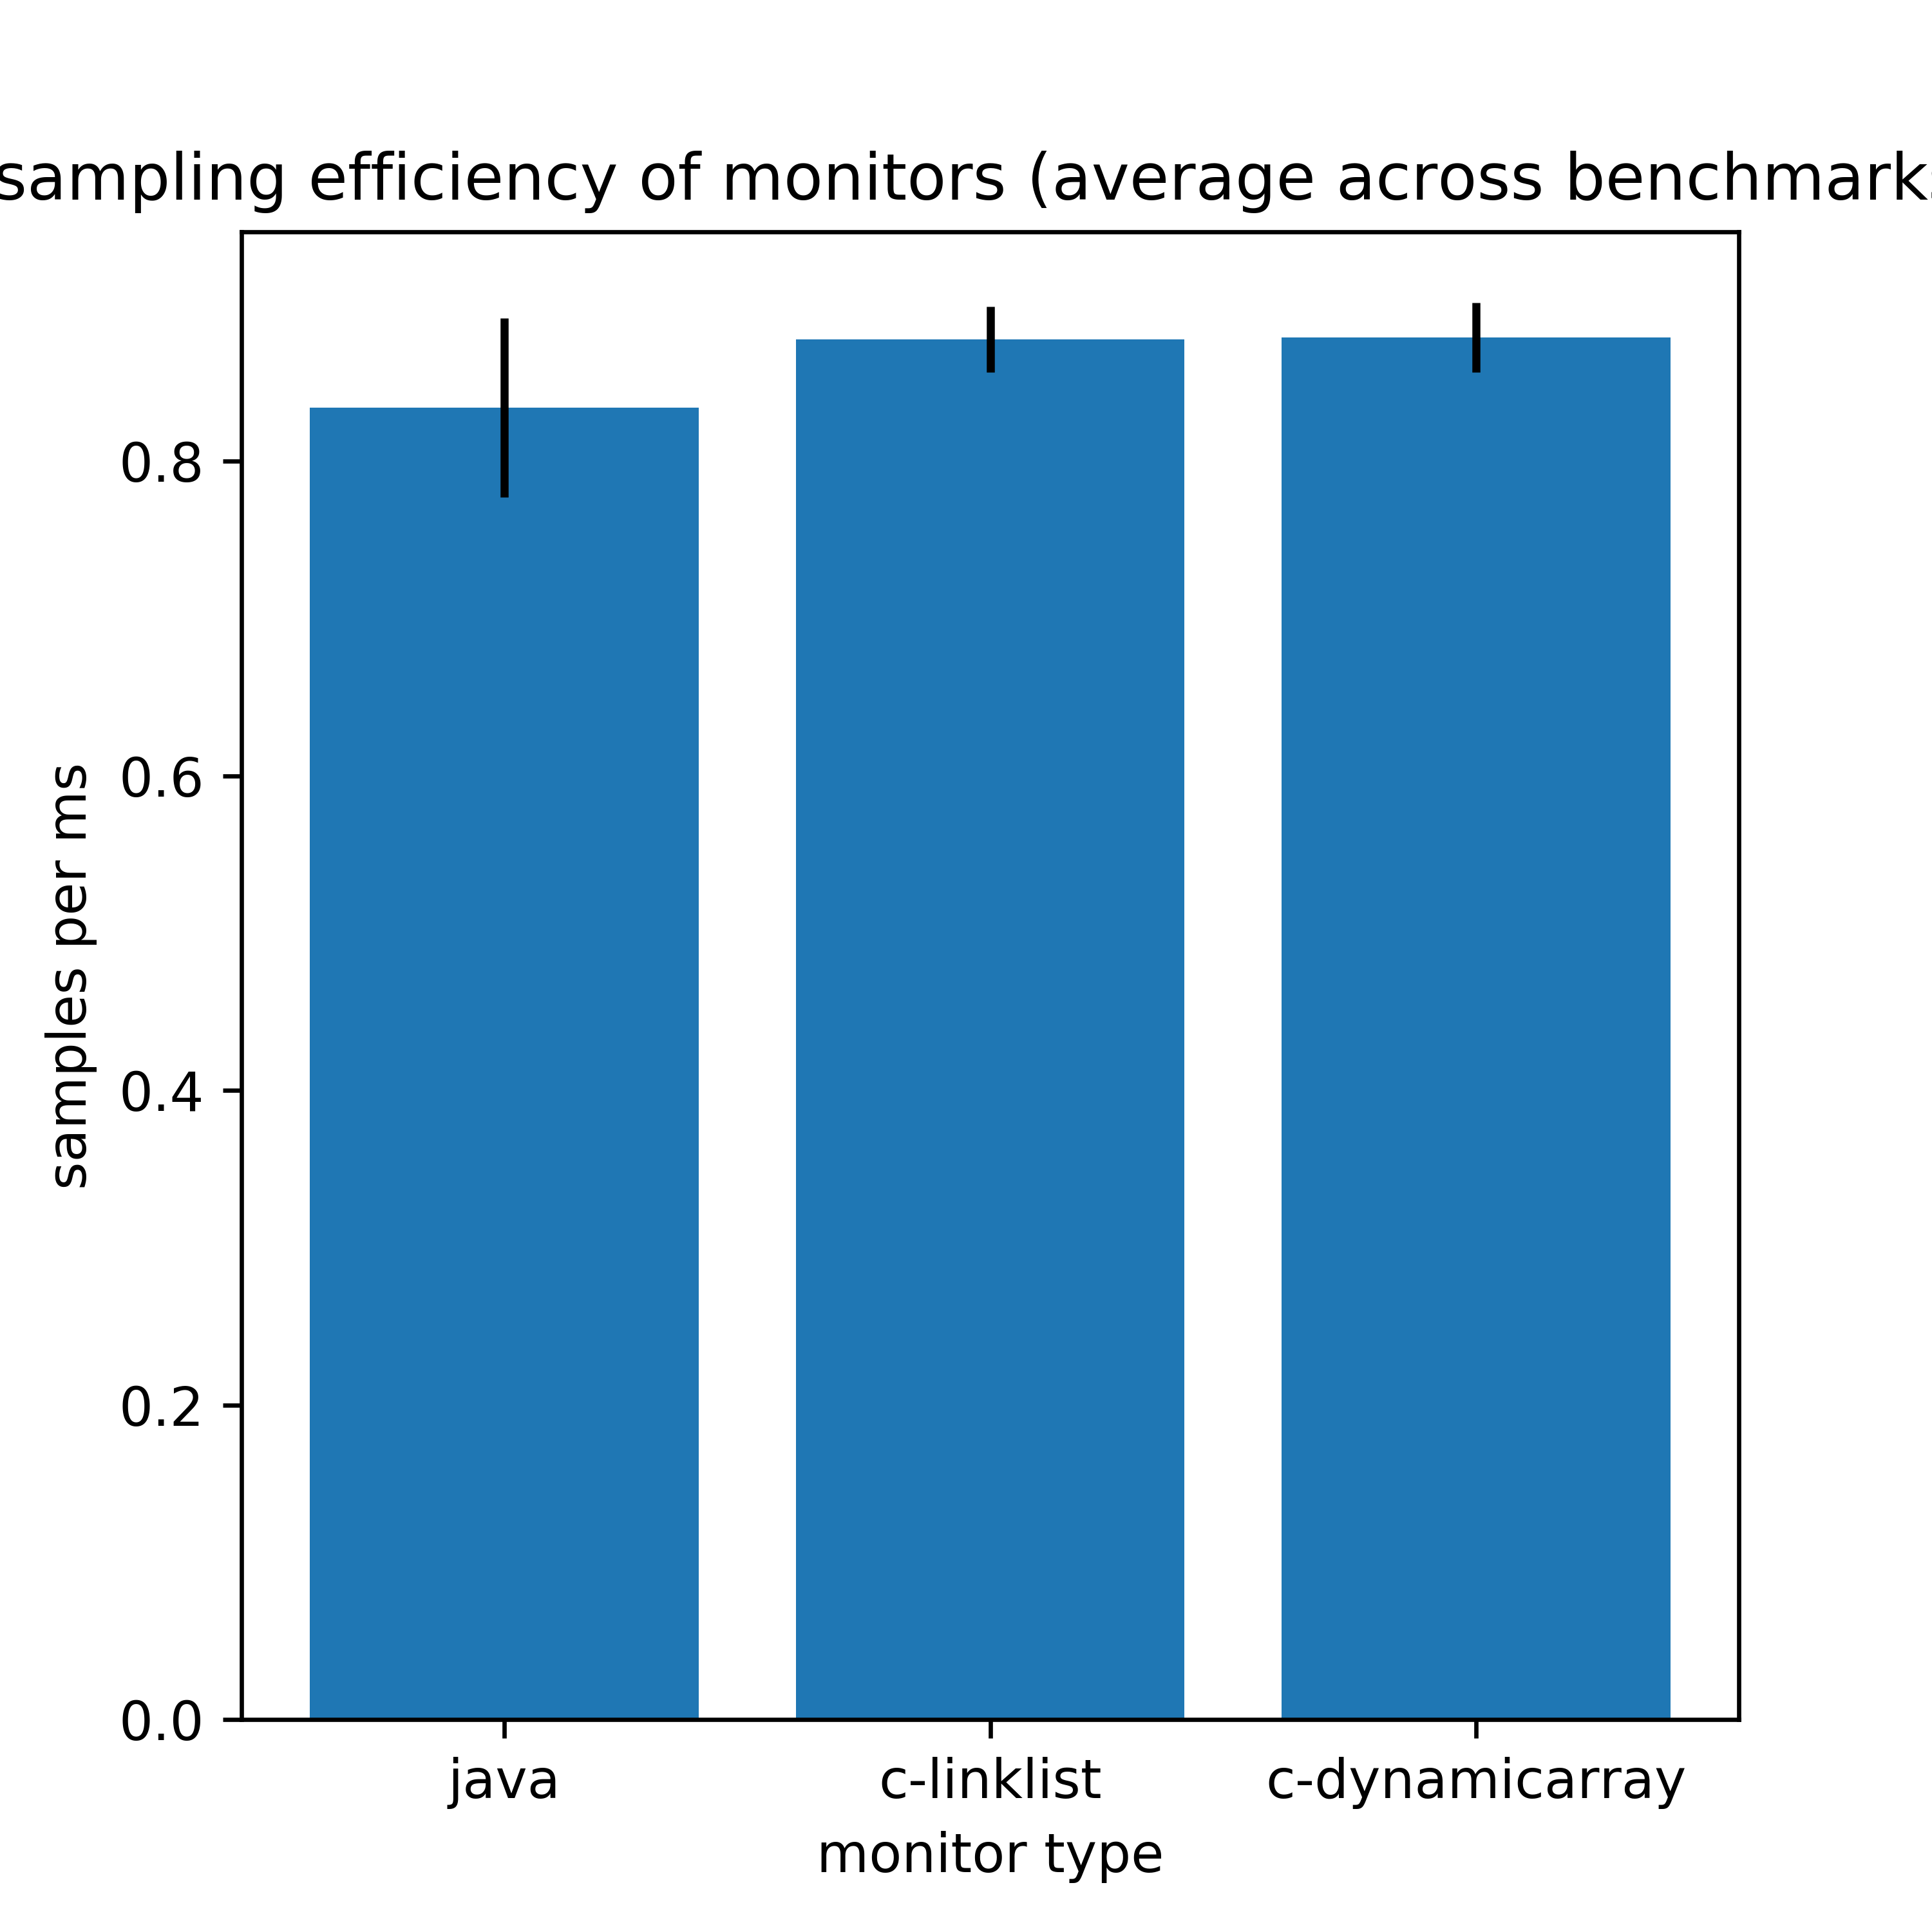
\includegraphics[width=17cm,height=17cm,keepaspectratio]{AsyncMonitorCompares/sampling-efficiency_overall.png}
    	\caption{Average sampling effieicency across all benchmarks}
    	\label{fig:samplingefficiency_overall}
    \end{figure}

Looks like Java is (slightly) less efficient, since sampling takes longer, as evidenced by
our JNI runtime overhead experiment. The wider error bar on the Java monitor makes sense. Looks
like it's a bit less precise in its sampling rate then.

\begin{verbatim} 
Raw Numbers
overall_java_avg: 0.8339
overall_java_std: 0.0569

overall_c_ll_avg: 0.8775
overall_c_ll_std: 0.0210

overall_c_da_avg: 0.8786
overall_c_da_std: 0.0222
\end{verbatim} % in case the actual numbers are useful at all

In conclusion, the C monitors are comparable in sampling efficiency, and both a bit better than
the Java one.

\subsection{Memory Footprint}
\anote{These results are definitely not accurate. I figured out some issues in my calculations, and the results are different. However, I can't upload the complete results because Jolteon is down. I have 3 iterations saved on my machine as standin data while I write my scripts, but data for all 25 iterations is currently unreachable until Jolteon gets fixed, so I can't run the analysis there and get new results.}

Below graph is the percent difference of memory added by having the AsyncEnergyMonitor active vs no monitor active. This is an average across all benchmarks.

    \begin{figure}[H]
    	\centering
    	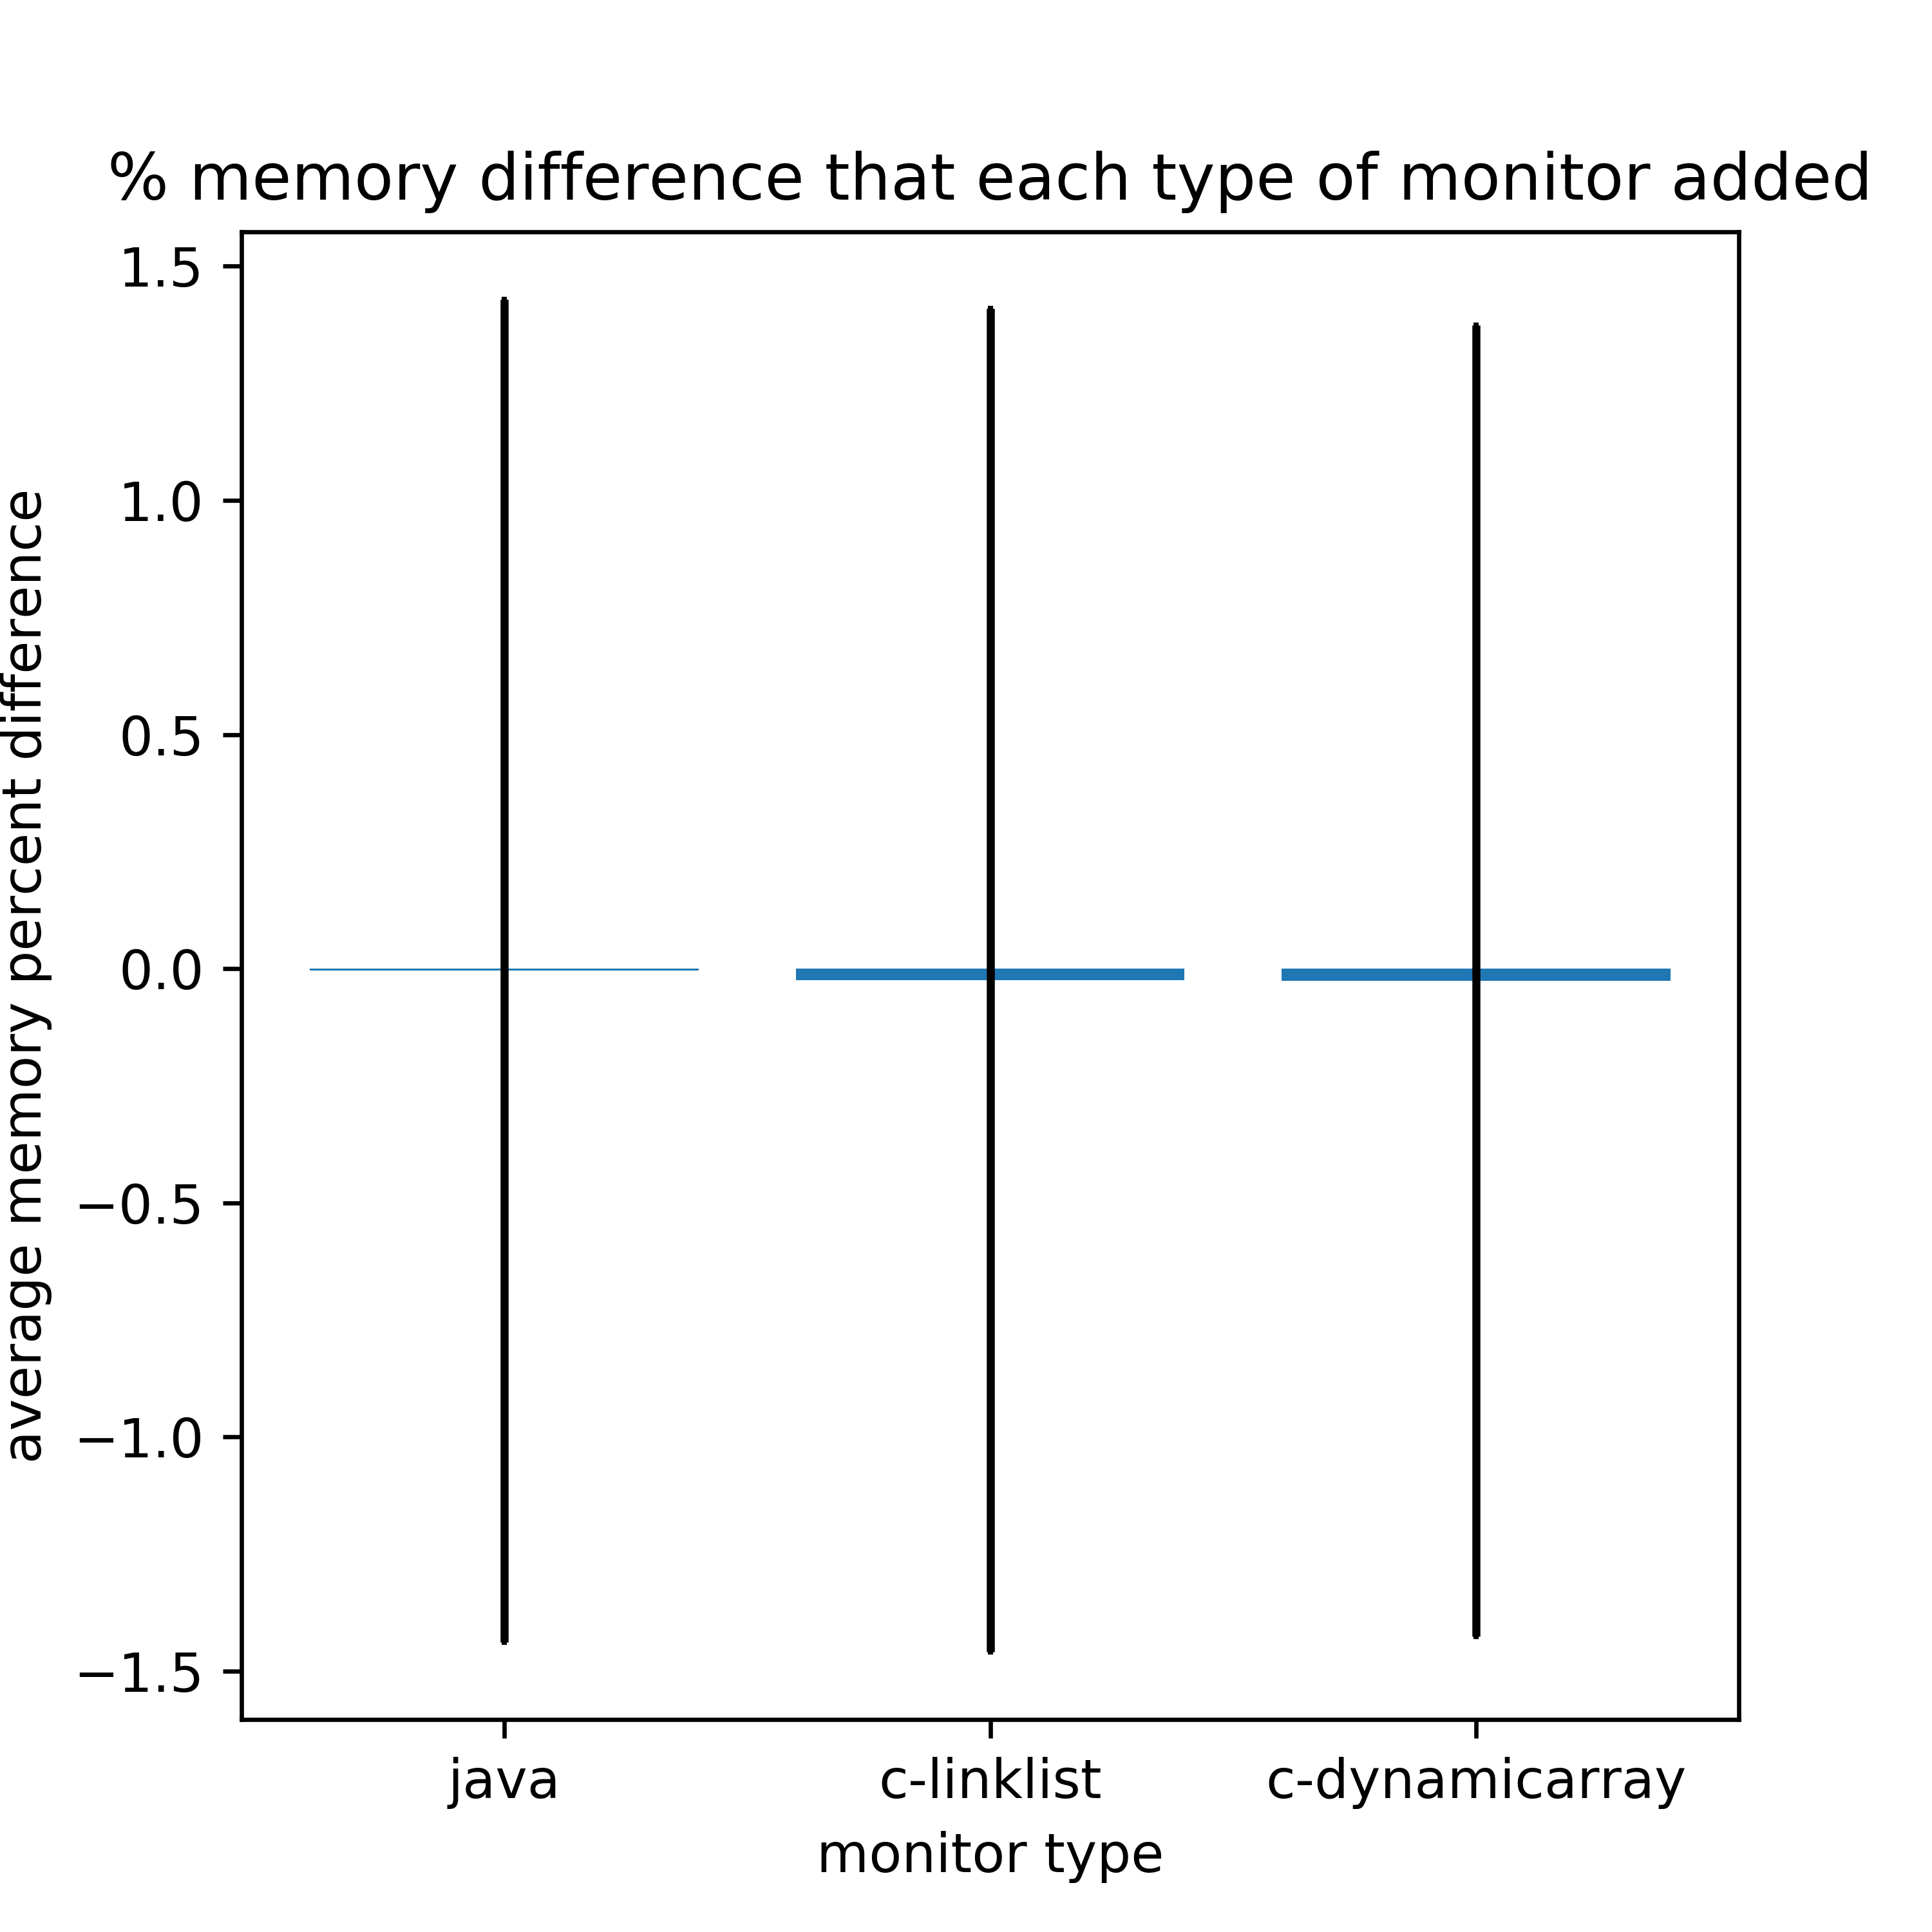
\includegraphics[width=17cm,height=17cm,keepaspectratio]{AsyncMonitorCompares/memory-compare_overall.png}
    	\caption{Memory Overhead of Each Monitor Type}
    	\label{fig:samplingefficiency_perbench}
    \end{figure}

The difference between the monitors (and the overall memory footprint) is extraordinarily negligible. This makes sense, since an energy monitor is effectively just a list of numbers in memory, it's just more fancy seeming because it gets updated asynchronously. But it's just energy readings and timestamps, so it's small potatoes in the grand scheme of things.

\anote{So the C monitors do tend have a slightly lower footprint, since a C sample stored in the monitor is a struct, while the Java sample is the string returned from native memory (if we parsed it into a primitive sample, it would have lower memory footprint but each sample would take even longer to generate). But as this experiment shows, it's all small potatoes compared to the total memory consumption of the benchmarks. So, is the smaller C memory worth writing about? Are there super memory sensitive Java situations that this is notable for?}

\anote{Should I talk about and try to explain the negative percent differences? Both the C monitors are slightly below 0...}